\graphicspath{{5Fractals/asy/}}

\section{Fractal Geometry}

\subsection{Natural Geometry, Self-similarity and Fractal Dimension}\label{sec:fracdefn}

Classical geometry typically considers objects (lines, curves, spheres, etc.) which seem flatter and less interesting as one zooms in: a differentiable curve at small scales looks like a line segment!\smallbreak
By contrast, real-world objects tend to exhibit greater detail at smaller scales. A seemingly spherical orange is dimpled on closer inspection. Is its surface area that of a sphere, or is it greater due to the dimples? What if we zoom in further? Under a microscope, the dimples are seen to have minute cracks and fissures. With modern technology, we can see almost to the molecular level; what does \emph{surface area} even mean at such a scale?

\boldinline{The Length of a Coastline} In 1967 Benoit Mandelbrot asked a related question in a now-famous paper, \emph{How Long Is the Coast of Britain?\ Statistical Self-Similarity and Fractional Dimension.} His essential point was that the question has no simple answer:\footnote{The official answer from the Ordnance Survey (the UK government mapping office) is, `It depends.' The all-knowing CIA states 7723 miles, though offers no evidence as to why.} Should one measure by walking along the mean high tide line? But where is this? Do we `walk' round every pebble? Round every grain of sand? Every molecule? As one shrinks the scale, the measured length becomes absurdly large. We sketch Mandelbrot's approach.\footnote{For more detail see the Fractal Foundation's \href{http://fractalfoundation.org/OFC/OFC-10-4.html}{website.} Mandelbrot coined the word \emph{fractal}, though he didn't invent the concept from nothing. Rather he applied earlier ideas of Hausdorff, Minkowski and others, and observed how the natural world contains many examples of fractal structures.}
\begin{itemize}%\itemsep0pt
  \item Given a ruler of length $R$, measure how many $N$ are required to trace round the coastline when laid end-to-end.
  \item Plotting $\log N$ against $\log (1/R)$ for several sizes of ruler seems to give a straight line!
  \[\log N\approx \log k+D\log(1/R)=\log (kR^{-D})\implies N\approx kR^{-D}\]
  The number $D$ is Mandelbrot's \emph{fractal dimension} of the coastline.
\end{itemize}

Mandelbrot's fractal dimension is purely empirical, though it does seem to capture something about the `bumpiness' of a coastline: the bumpier, the greater its fractal dimension. For mainland Britain with its smooth east and rugged west coasts, $D\approx 1.25$. Given its many fjords, Norway has a far rougher coastline and a higher fractal dimension $D\approx 1.52$.

\begin{example}[lower separated=false, sidebyside, sidebyside align=top seam, sidebyside gap=0pt, righthand width=0.29\linewidth]{}{}
As a sanity check, consider a smooth circular `coastline.' Approximate the circumference using $N$ rulers of length $R$: clearly
\[R=2\sin\frac\pi N\]
As $N\to\infty$, the small angle approximation for sine applies,
\[R\approx \frac{2\pi}N\implies N\approx 2\pi R^{-1}\]
where the approximation improves as $N\to\infty$. The fractal dimension of a circle is therefore 1.
\tcblower
\flushright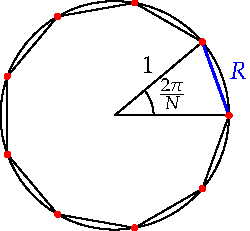
\includegraphics{circle}
\end{example}
\goodbreak


Our goal is to describe self-similar objects and thus create a new notion of dimension related to Mandelbrot's. To begin consideration of self-similarity, we first consider some of the standard objects of pre-fractal geometry.\par
\begin{minipage}[t]{0.75\linewidth}\vspace{-5pt}
\begin{description}
	\item[Line] A \textcolor{Green}{segment} can be viewed as $N$ copies of itself scaled by a factor $r=\frac 1N$.
	\item[Square] A \textcolor{blue}{square} comprises $N$ copies of itself scaled by a factor $r=\frac 1{\sqrt N}$.
	\item[Cube] A cube comprises $N$ copies of itself scaled by a factor $r=\frac 1{\sqrt[3]{N}}$.
\end{description}\vspace{-5pt}
In each case observe that $N=\left(\frac 1r\right)^D$ where $D$ is the usual dimension of the object (1, 2 or 3). Inspired by this, we make a loose definition.
\end{minipage}\hfill\begin{minipage}[t]{0.24\linewidth}\vspace{-15pt}
\flushright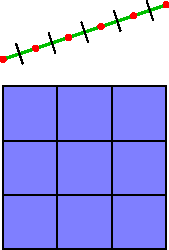
\includegraphics[scale=0.95]{self-sim-line}
\end{minipage}


\begin{defn}{}{selfsim}
A geometric figure is \emph{self-similar} if it may be subdivided into $N$ similar copies of itself, each scaled by a magnification factor $r<1$. The \emph{fractal dimension} of such a figure is
\[\displaystyle D:=\log_{1/r}N=\frac{\log N}{\log (1/r)}=-\frac{\log N}{\log r}\]
\end{defn}


\begin{example}{}{}
The botanical pictures below offer some evidence for non-integer fractal dimension and that self-similarity is a natural phenomenon. The `tree' comprises
%\footnote{Because of the construction, including translating the picture, the whole contains a little more than three copies of itself. The bottom part of the stem and the largest two green branches are `extra.' This is of no import.}
 $N=3$ copies of itself, each scaled by a factor of $r=0.4$. Its fractal dimension is $D=-\frac{\log 3}{\log 0.4}\approx 1.199$.\par
The fern has $N=7$ and $r=0.3$ for a fractal dimension $D=-\frac{\log 7}{\log 0.3}\approx 1.616$.

\begin{center}
\begin{tabular}{c@{\qquad\qquad}c}
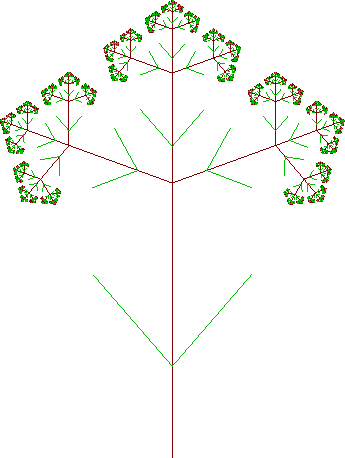
\includegraphics{tree2}
&
\href{http://www.math.uci.edu/~ndonalds/math161/fern-code.html}{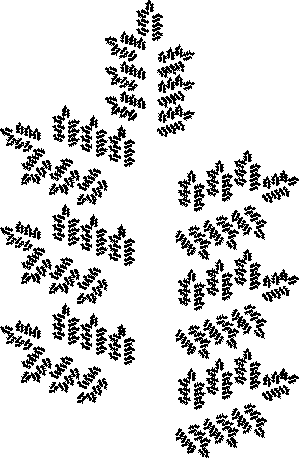
\includegraphics{tree3}}
\\
Tree fractal $D\approx 1.199$
&
Fern fractal $D\approx 1.616$
\end{tabular}
\end{center}%\smallbreak
The pictures illustrate the interpretation of fractal dimension. Both objects seem to occupy more space than mere lines, but neither has positive area. Moreover, the fern seems to occupy more space than the tree. The `trunk' and `branches' in the first picture aren't part of the fractal; we've drawn them only to give the picture a skeleton. The fern, without stalks, is a more accurate approximation of a fractal. 
\end{example}


\goodbreak


\begin{example}{Cantor's Middle-third Set}{cantor}
This famous example dates from the late 1800s.\footnotemark{}\par
\begin{minipage}[t]{0.58\linewidth}\vspace{-5pt}
Starting with the unit interval $C_0=[0,1]$, define a sequence of sets $(C_n)$ where $C_{n+1}$ is obtained by deleting the open `middle-third' of each interval in $C_n$; for instance
\[C_1=\left[0,\frac 13\right]\cup\left[\frac 23,1\right]\]
Cantor's set is essentially the limit of this sequence:
\[\mathcal C:=\bigcap_{n=0}^\infty C_n\]
\end{minipage}\hfill\begin{minipage}[t]{0.4\linewidth}\vspace{-7pt}
\flushright
\href{http://www.math.uci.edu/~ndonalds/math161/cantor-similar.html}{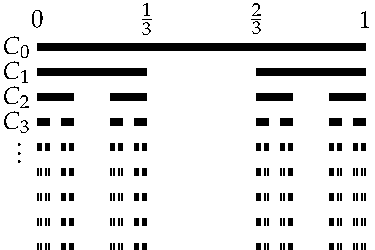
\includegraphics{cantor-set}}
\end{minipage}\medbreak

It has several strange properties\ldots
\begin{description}%\itemsep0pt
  \item[Zero length] If the \emph{length} of a set is the sum of the lengths of its disjoint sub-intervals, then
	\[\operatorname{length}(C_n)=\left(\frac 23\right)^n\]
	since we delete $\frac 13$ of the remaining set at each step. It follows that
  \[\forall n\in\N_0,\ \operatorname{length}(\mathcal C)\le \left(\frac 23\right)^n \implies \operatorname{length}(\mathcal C)=0\]
  Otherwise said, $\mathcal C$ contains no subintervals.
  \item[Uncountable] There exists a bijection between $\mathcal C$ and the original interval $[0,1]$!
  \item[Self-similarity] Abusing notation somewhat,
	\[C_{n+1}=\frac 13C_n\cup\left(\frac 13C_n+\frac 23\right)\]
	where we mean that $C_{n+1}$ consists of two copies of $C_n$, each shrunk by a factor of $\frac 13$ and one shifted $\frac 23$ to the right. The upshot is that the Cantor set itself satisfies
	\[\mathcal C=\frac 13\mathcal C\cup\left(\frac 13\mathcal C+\frac 23\right)\]
	Being similar to two disjoint subsets of itself, its fractal dimension is $D=\frac{\log 2}{\log 3}\approx 0.631$. The above image links to an animation showing how the full set may be doubled to produce itself.
\end{description}

The Cantor set has many generalizations. Look up the \href{https://en.wikipedia.org/wiki/Sierpiński_triangle}{Sierpiński triangle} ($D=\smash{\frac{\log 3}{\log 2}}\approx 1.585$) and carpet (Examples \ref{ex:scarpet}, $D=\frac{\log 8}{\log 3}\approx 1.893$), and the Menger sponge ($D=\frac{\log 20}{\log 3}\approx 2.727$).
\end{example}

\footnotetext{Henry Smith discovered it in 1874 while investigating integrability; in this context, the `length' of a set was later formalized using \emph{measure theory.} Cantor's description in 1883 was more focused on topological properties. Self-similarity was less of a concern at the time.}

\goodbreak


\begin{example}{The Koch Curve and Snowflake}{koch}
The Koch curve is another generalization of the Cantor set, produced as the limit of a sequence of curves.\par
\begin{minipage}[t]{0.64\linewidth}\vspace{-5pt}
\begin{itemize}\itemsep0pt
  \item Let $K_0$ be a segment of length 1.
  \item Replace the middle third of $K_0$ with the other two sides of an equilateral triangle to create $K_1$.
  \item Replacing the middle third of each segment in $K_1$ as before to create $K_2$.
  \item Repeat this process \emph{ad infinitum.}
\end{itemize}
The curve is drawn, along with the \emph{Koch snowflake} obtained by arranging three copies around an equilateral triangle.\smallbreak

The relation to the Cantor set should be obvious in the construction. Indeed if $K_0=[0,1]$, then the intersection of this with the Koch curve is the Cantor set!\smallbreak

The Koch curve is self-similar in that it comprises $N=4$ copies of itself shrunk by a factor of $r=\frac 13$. Its fractal dimension is therefore $\frac{\log 4}{\log 3}\approx 1.2619$.\smallbreak

We may also consider the curve's length. Let $s_n$ be the number of segments in $K_n$, each having length $t_n$. Also let $\ell_n=t_ns_n$ be the length of the curve $K_n$. We easily see that
\begin{gather*}
  s_n=4^n,\quad t_n=\frac 1{3^n}\implies \ell_n=\left(\frac 43\right)^n\to\infty
\end{gather*}
from which the Koch curve is \emph{infinitely long}!
\end{minipage}\hfill\begin{minipage}[t]{0.35\linewidth}\vspace{-15pt}
\flushright
\href{http://www.math.uci.edu/~ndonalds/math161/koch-anim.html}{
\begin{tabular}{@{}c@{}}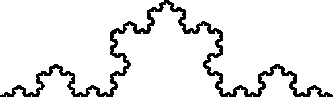
\includegraphics{koch}\\
Koch Curve\\[8pt]
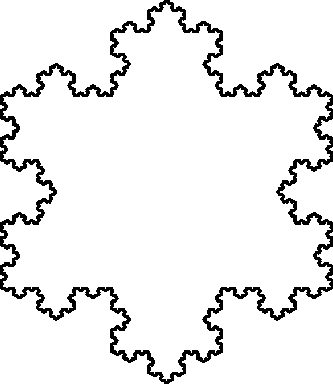
\includegraphics{koch2}\\
Koch Snowflake\\[8pt]
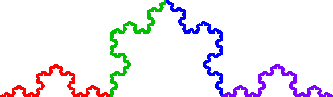
\includegraphics{koch3}\\
Self-similarity
%\animategraphics[controls]{1}{_kochanim3}{0}{6}\\
%\animategraphics[controls,poster=last]{1}{_kochanim2}{0}{6}
\end{tabular}
}
\end{minipage}
\end{example}



\begin{exercises}
\exstart By removing a constant middle fraction of each interval, construct a fractal analogous to the Cantor set but with dimension $\frac 12$.

\begin{enumerate}\setcounter{enumi}{1}\itemsep2pt
	\item Prove that the area inside the $n\th$ iteration of the construction of the Koch snowflake is
	\[A_n=\left(1+\frac 35\left[1-\left(\frac 49\right)^n\right]\right)\frac{\sqrt 3}{4}\]
	\emph{The area inside the complete snowflake is therefore $\frac 85$ that of the original triangle.}
	
	\item Suppose $\vr(t)$, $t\in [0,1]$ is a regular (smooth) curve in the plane.
	\begin{enumerate}
  	\item Use the arc-length formula $L=\int_0^1\nm{\vr'(t)}\,\dt$ together with Riemann sums and the linear approximation $\vr(t+\epsilon)\approx\vr(t)+\epsilon\vr'(t)$ with $\epsilon=\frac 1N$ to argue that
  	\[L\approx\sum_{k=0}^{N-1}\nm{\vr\left(\frac{k+1}N\right)-\vr\left(\frac{k}N\right)} \tag{$\ast$}\]

  	\item Suppose the curve is parametrized such that each segment on the right side of $(\ast)$ has the same length $R$. Prove that $L\approx NR$.\par
  	\emph{Any regular curve thus has fractal dimension 1 in the sense stated by Mandelbrot (pg.\,\pageref{sec:fracdefn}).}  
	\end{enumerate}
	
\end{enumerate}
\end{exercises}


\clearpage




\subsection{Contraction Mappings \& Iterated Function Systems}

Thus far we have only dealt with fractals where the whole consists of pieces scaled by the same factor. In general we can mix up scaling factors. To do this it is helpful to borrow some language from topology.

\begin{defn}{}{}
A \emph{contraction mapping} is a function $S$ on a subset of $\R^n$ such that $\exists c\in[0,1)$ with
\[\nm{S(x)-S(y)}\le c\nm{x-y}\]
\end{defn}

A contraction mapping therefore moves points closer together. It should be clear that every contraction mapping is continuous. The main idea of this section is that fractals may be generated by repeatedly applying contraction mappings to an initial shape. We have already seen a example:


\begin{example*}{\ref{ex:cantor}, mk.\,II}{}
Consider the following functions $S_1,S_2:\R\to\R$
\[S_1(x)=\frac x3\qquad S_2(x)=\frac x3+\frac 23\]
These are certainly contraction mappings
\[\forall x,y\in\R,\ \nm{S_1(x)-S_1(y)}=\nm{S_2(x)-S_2(y)}=\frac 13\nm{x-y}\]
with scale factor $c=\frac 13$. More importantly, these functions \emph{define} the Cantor set: at each stage of its construction, we have
\[C_{n+1}:=S_1(C_n)\cup S_2(C_n)\]
As the limit of this process, the self-similarity of the Cantor set can be expressed in the same manner: $\mathcal C=S_1(\mathcal C)\cup S_2(\mathcal C)$.\medbreak

Surprisingly, it barely seems to matter what initial set $C_0$ we choose. For example, we could start with the singleton set $C_0=\{0\}$, from which
\[C_1=\{0,\tfrac 23\},\qquad C_2=\{0,\tfrac 29,\tfrac 23,\tfrac 89\},\qquad C_3=\{0,\tfrac 2{27},\tfrac 29,\tfrac 8{27},\tfrac 23,\tfrac{20}{27},\tfrac 89,\tfrac{26}{27}\},\ \ldots\]
We draw the first few iterations below. In the second picture, we start with a very different initial set $C_0=[0.2,0.5]\cup[0.6,0.7]$. Iterating this also appears to produce the Cantor set!
\begin{center}
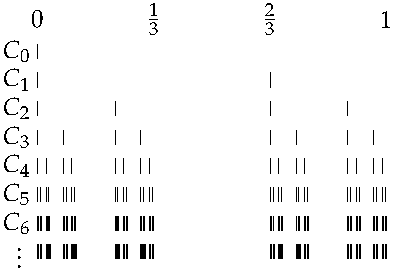
\includegraphics{cantor-similar3}
\qquad\qquad
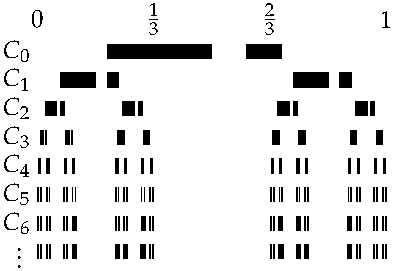
\includegraphics{cantor-similar2}
\end{center}
\end{example*}

\goodbreak


\boldsubsubsection{Iterated Function Systems}

It certainly seems as if the Cantor set might be generated by the contraction maps $S_1,S_2$ independently of the initial data $C_0$. The following result shows in what sense this is the case, though it relies on some heavy lifting from topology. If you've done some analysis, then several of the concepts will be familiar. We summarize the discussion without proof.

\begin{itemize}
  \item A subset of $\R^m$ is \emph{compact} if it is \emph{closed} (contains its boundary points) and \emph{bounded} (all points lie within some ball centered at the origin).
  
  \item The set of all compact subsets of $\R^m$ is a metric space $\mathcal H$. This means that the \emph{distance} $d(X,Y)$ between two compact sets $X,Y\in\mathcal H$ may sensibly be defined, though it is a little tricky\ldots\footnote{This is the \emph{Hausdorff metric.} Given $Y\in\mathcal H$, and $x\in \R^n$, define $d_Y(x)=\inf_{y\in Y}\Nm{x-y}$ to be the distance from $x$ to the `nearest' point of $Y$. Define $d_X(y)$ similarly. The Hausdorff distance between $X$ and $Y$ is then
  \[d(X,Y):=\max\left\{\sup_{x\in X}d_Y(x),\sup_{y\in Y}d_X(y)\right\}\]
  Roughly speaking, find $x\in X$ which is as far away $d_Y(x)$ as possible from anything in $Y$, and find $y\in Y$ similarly; $d(X,Y)$ is the larger of these distances.}
  
  \item Since $\mathcal H$ is a metric space, we can discuss convergent sequences $(K_n)$ of compact sets
	\[\lim_{n\to\infty}K_n=K\iff \lim_{n\to\infty}d(K_n,K)=0\]
	It also makes sense to speak of Cauchy sequences in $\mathcal H$. Moreover, $\mathcal H$ is \emph{complete} in that every Cauchy sequence $(K_n)\subseteq\mathcal H$ converges to some $K\in\mathcal H$.
	
  \item The \emph{Banach Fixed Point Theorem} now applies.
  \begin{quote}
  {If $S:\mathcal H\to\mathcal H$ is a contraction mapping on a complete metric space $\mathcal H$, then $S$ has a unique fixed point (some $F\in\mathcal H$ such that $S(F)=F$). Moreover, if $F_0\in\mathcal H$ is any initial value, then the sequence defined iteratively by $F_{k+1}=S(F_k)$ converges to $F$.}
  \end{quote}
  This powerful result has applications throughout mathematics.
\end{itemize}


\begin{thm}{}{ifs}
Let $S_1,\ldots,S_n$ be contraction mappings on $\R^m$ with ratios $c_1,\ldots,c_n$. Define
\[S:\mathcal H\to\mathcal H\quad\text{by}\quad S(D)=\bigcup_{i=1}^nS_i(D)\]
\begin{enumerate}
  \item $S$ is a contraction mapping on $\mathcal H$, with contraction ratio $c=\max\{c_i\}$.
  \item $S$ has a unique fixed set $F\in\mathcal H$ given by $F=\lim\limits_{k\to\infty} S^k(E)$ for any non-empty $E\in\mathcal H$.
\end{enumerate}
\end{thm}

Part 1 is not difficult to prove if you're willing to work with the definition of the Hausdorff metric (try it if you're comfortable with analysis!). Part 2 is Banach's theorem.\smallbreak

The upshot is this: if we take any non-empty compact set $E$ and repeatedly apply contraction mappings, the process will converge to a limit which is \emph{independent of $E$!} We call the limit set $F$ for \emph{fractal.} Such fractals are often called \emph{attractors}: being limit-sets, they `attract' data towards themselves.

\goodbreak


\begin{examples}{}{scarpet}
\exstart (Cantor set Ex.\,\ref{ex:cantor})\lstsp Theorem \ref{thm:ifs} shows that we may let $C_0$ be \emph{any} closed bounded subset of $\R$. Repeatedly applying the contraction mappings $S_1$ and $S_2$ will always result in the same set $\mathcal C$.\vspace{-10pt}

\begin{enumerate}\setcounter{enumi}{1}
  \item[]A nice application is that one can easily find all sorts of interesting points in the Cantor set. For instance, suppose $x,y\in\R$ are a pair such that $y=S_1(x)$ and $x=S_2(y)$: otherwise said
\[y=\frac 13 x\quad\text{and}\quad x=\frac 13(y+2)\]
Since $E=\{x,y\}$ is a compact set satisfying $E\subseteq S(E)$, it follows that $E\subseteq\lim%\limits_{k\to\infty}
S^k(E)=\mathcal C$, from which $x,y$ both lie in the Cantor set! However, we can easily solve to see that $(x,y)=(\frac 34,\frac 14)$. This seems paradoxical: $\frac 14$ does not lie at the end of any deleted interval (denominators of the form $3^n$) but yet the Cantor set contains no intervals. How does $\frac 14$ end up in there?!

\begin{minipage}[t]{0.65\linewidth}\vspace{0pt}
	\item (Koch curve, Ex.\,\ref{ex:koch})\lstsp Define four mappings $S_i:\R^2\to\R^2$, each with scale factor $c=\frac 13$.
\end{minipage}\hfill\begin{minipage}[t]{0.34\linewidth}\vspace{0pt}
	\flushright \href{http://www.math.uci.edu/~ndonalds/math161/koch-anim2.html}{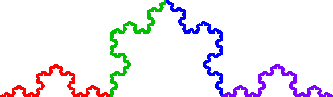
\includegraphics[scale=0.96]{koch3}}
\end{minipage}\par
\vspace{-15pt}

$\renewcommand\arraystretch{1.4}
\begin{array}{l|l}
\text{Mapping}&\text{Effect}\\\hline
\displaystyle S_1(x,y)=\left(\tfrac x3,\tfrac y3\right)&\text{Scale $\frac 13$}\\
\displaystyle S_2(x,y)=\left(\tfrac 16x-\tfrac{\sqrt 3}6y+\tfrac 13,\tfrac{\sqrt 3}6x+\tfrac 16y\right) &\text{Scale $\frac 13$, rotate \ang{60}, translate}\\
\displaystyle S_3(x,y)=\left(\tfrac 16x+\tfrac{\sqrt 3}6y+\tfrac 12,\tfrac{\sqrt 3}6x-\tfrac 16y+\tfrac{\sqrt 3}6\right) &\text{Scale $\frac 13$, rotate $-\ang{60}$, translate}\\
\displaystyle S_4(x,y)=\left(\tfrac x3+\tfrac 23,\tfrac y3\right) &\text{Scale $\frac 13$, translate}
\end{array}$\par
Applied to the Koch curve, the image of each map corresponds by color. The picture links to a series of animated constructions of the curve starting with different initial sets $E$.

\begin{minipage}[t]{0.72\linewidth}\vspace{0pt}
	\item (Sierpiński carpet)\lstsp Eight contraction mappings produce this fractal, each reducing the whole by a (length-scale) factor of $\frac 13$.\smallbreak
As with the Koch curve, the image links to several alternative constructions using different initial starting sets.
\end{minipage}
\hfill
\begin{minipage}[t]{0.27\linewidth}\vspace{0pt}
	\flushright \href{http://www.math.uci.edu/~ndonalds/math161/sier-anim.html}{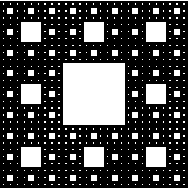
\includegraphics[scale=1]{sieranim2}}
\end{minipage}\par


\begin{minipage}[t]{0.72\linewidth}\vspace{0pt}
	\item (A Fractal Fern)\lstsp This is built from three contraction mappings:
	\begin{itemize}
		\item[$S_1$:] Scale by $\frac 34$, rotate \ang{5} clockwise, and translate by $(0,\frac 14)$
		\item[$S_2$:] Scale by $\frac 14$, rotate \ang{60} counter-clockwise, and translate by $(0,\frac 14)$
		\item[$S_3$:] Scale by $\frac 14$, rotate \ang{60} clockwise, and translate by $(0,\frac 14)$
	\end{itemize}
\end{minipage}
\hfill
\begin{minipage}[t]{0.27\linewidth}\vspace{0pt}
	\flushright \href{http://www.math.uci.edu/~ndonalds/math161/fern-anim.html}{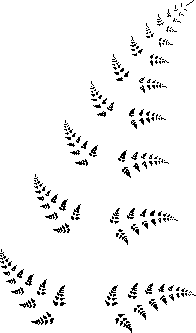
\includegraphics[scale=1]{fern2}}
\end{minipage}

\end{enumerate}
\end{examples}

\goodbreak




\begin{minipage}[t]{0.8\linewidth}\vspace{0pt}
\boldsubsubsection{Fractal Dimension Revisited}

Since Theorem \ref{thm:ifs} permits several different contraction factors, we need a new approach to computing fractal dimension. We ask how many disks of a given radius $\epsilon$ are required to cover a set. In the picture, the \textcolor{blue}{unit square} requires four disks of radius $\varepsilon=0.4$. For smaller $\varepsilon$, we will plainly need more disks\ldots
\end{minipage}
\hfill
\begin{minipage}[t]{0.19\linewidth}\vspace{0pt}
\flushright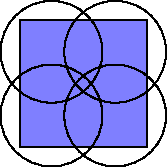
\includegraphics{epsiloncover}
\end{minipage}


\begin{defn}{}{}
Let $A$ be a compact subset of $\R^m$.
\begin{enumerate}
  \item If $\varepsilon>0$, the \emph{closed $\varepsilon$-ball centered at $x\in A$} consists of the points at most a distance $\varepsilon$ from $x$:
	\[B_\epsilon(x)=\{y\in\R^m:d(x,y)\le\varepsilon\}\]
% 	\item A finite union $\smash{\bigcup\limits_{n=1}^MB(x_n,\varepsilon)}$ is an \emph{$\varepsilon$-covering} of $A$ if $A\subseteq \smash{\bigcup\limits_{n=1}^MB(x_n,\varepsilon)}$: that is,
% 	\[\forall x\in A,\ \exists n\ \text{ such that }\ x\in B(x_n,\varepsilon)\]
	\item The \emph{minimal $\varepsilon$-covering number} for $A$ is
	\[\mathcal N(A,\varepsilon)=\min\left\{M:\exists x_1,\ldots,x_M\in A\text{ with }A\subseteq \bigcup\limits_{n=1}^MB_\epsilon(x_n)\right\}\]
	
	\item Given a compact set $A\subseteq\R^m$, its \emph{fractal dimension} is the limit
\[D=\lim_{\varepsilon\to 0}\frac{\log\mathcal N(A,\varepsilon)}{\log (1/\varepsilon)}\]
\end{enumerate}
\end{defn}

We don't claim to prove that $D$ must exist, though a simple example should at least convince you that the definition is reasonable!

\begin{example}{}{intervalcover}
Let $A=[0,1]$ be the interval of length 1. It is not hard to see that
\[\varepsilon\ge\frac 12\iff \cN(\varepsilon)=1,\quad\text{and}\quad \frac 14\le \varepsilon<\frac 12\iff \cN(\varepsilon)=2\]
etc. More generally, $\cN$ and $\epsilon$ are related via
\[\frac 1{2\cN}\le\epsilon<\frac 1{2(\cN-1)}\]
% \[\def\arraystretch{1.3}\begin{array}{c|c}
% \text{range of }\varepsilon&\mathcal N([0,1],\epsilon)\\\hline
% \frac 12\le \varepsilon&1\\
% \frac 14\le\varepsilon<\frac 12&2\\
% \frac 16\le\varepsilon<\frac 14&3\\
% \frac 18\le\varepsilon<\frac 16&4\\
% \frac 1{10}\le\varepsilon<\frac 18&5\\
% \frac 1{2m}\le\varepsilon<\frac 1{2(m-1)}&m
% \end{array}\]
% \[\begin{array}{c|ccccccc}\def\arraystretch{1.3}
% \text{range of }\varepsilon & [\frac 1{2m},\frac 1{2(m-1)}) & \cdots & [\frac 1{10},\frac 18) & [\frac 18,\frac 16) & [\frac 16,\frac 14) & [\frac 14,\frac 12) & [\frac 12,\infty)\\\hline
% \mathcal N([0,1],\epsilon) & m & \cdots & 5 & 4 & 3 & 2 & 1
% \end{array}\]
The dimension of the line (1) may therefore be recovered via the squeeze theorem
\[%\frac{\log\mathcal N}{\log (2\cN)} <\frac{\log\mathcal N}{\log (1/\varepsilon)}< \frac{\log\mathcal N}{\log (2(\cN-1))}  \implies 
D=\lim_{\epsilon\to 0}\frac{\log\mathcal N}{\log (1/\varepsilon)}=1\]
%A similar trick happens in other dimensions, though it is harder to compute explicitly.
\end{example}



Thankfully an easier-to-use modification is available using boxes.

\begin{thm}[breakable]{Box-counting}{}
Let $A$ be compact and cover $\R^m$ by boxes of side length $\frac 1{2^n}$. Let $\mathcal N_n(A)$ be the number of boxes intersecting $A$. Then
\[D=\lim_{n\to\infty}\frac{\log\mathcal N_n(A)}{\log 2^n}\]
\end{thm}

\goodbreak

We finish with a formula satisfied by the dimension of an iterated function system (Theorem \ref{thm:ifs}).
% The idea is is essentially to trap the number of boxes covering $A$ between two sequences of $\varepsilon$-balls and apply the squeeze theorem.

\begin{thm}{}{ifsdimension}
Let $\{S_n\}_{n=1}^M$ be an iterated function system with attractor (limiting fractal) $F$ and where each contraction $S_n$ has scale factor $c_n\in(0,1)$. At each stage of the construction, suppose portions of the fractal generated by each contraction map meet only at boundary points. Then the fractal dimension is the unique $D$ satisfying
\[\sum_{n=1}^Mc_n^D=1\]
\end{thm}

\begin{examples}{}{}
\exstart If all scale-factors are identical $c_n=r$, we recover Definition \ref{defn:selfsim},
\[Mr^D=1\implies D=\frac{-\log M}{\log r}=\frac{\log M}{\log (1/r)}\]
\begin{enumerate}\setcounter{enumi}{1}
  \item The fractal fern (Examples \ref{ex:scarpet}) is generated by three contraction maps with scale factors $\frac 34,\frac 14,\frac 14$. Its dimension is the solution to the equation
  \[\left(\frac 34\right)^D+\left(\frac 14\right)^D+\left(\frac 14\right)^D=1\implies D\approx 1.3267\]
  \item Numerical approximation is usually required to solve for $D$, though sometimes an exact solution is possible. For instance, if $c_1=c_2=\frac 12$ and $c_3=c_4=c_5=\frac 14$, then
  \[2\left(\frac 12\right)^D+3\left(\frac 14\right)^D=1\]
  Writing $\alpha=\left(\frac 12\right)^D$ yields the quadratic equation
  \[2\alpha+3\alpha^2=1\implies \alpha=\frac 13\implies D=\log_23\approx 1.5849\]
\end{enumerate}
\end{examples}


\begin{minipage}[t]{0.58\linewidth}\vspace{0pt}
\boldsubsubsection{Other methods of creating fractals}

The contraction mapping approach is one of many ways to create fractals. Two other famous examples are the \href{https://en.wikipedia.org/wiki/Logistic_map}{\emph{logistic map}} (related to numerical approximations to non-linear differential equations) and the \href{https://en.wikipedia.org/wiki/Mandelbrot_set}{\emph{Mandelbrot set}} (pictured).\smallbreak
The Mandelbrot set arises from a construction in the complex plane. For a given $c\in\C$, we iterate the function
\[f_c(z)=z^2+c\]
If $f(f(f(\cdots f(c)\cdots)))$ remains bounded, no matter how many times $f$ is applied, then $c$ lies in the Mandelbrot set.\smallbreak
Much better pictures, and trippy videos can be found online\ldots
\end{minipage}
\hfill
\begin{minipage}[t]{0.4\linewidth}\vspace{0pt}
\flushright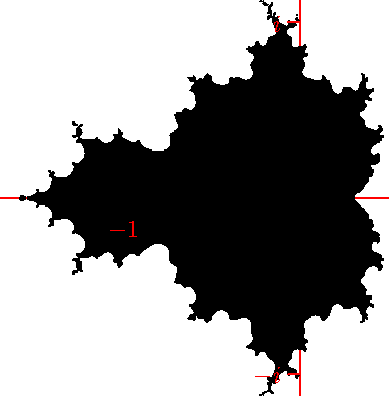
\includegraphics[scale=1]{mandelbrot}
\end{minipage}
\goodbreak



\begin{exercises}
\exstart Let $S_1(x)=\frac 13 x$ and $S_2(x)=\frac 13x+\frac 23$ be the contraction mappings defining the Cantor set and suppose $x,y,z\in\R$ satisfy
  \[y=S_1(x),\qquad z=S_2(y),\qquad x=S_2(z)\]
  Show that $x,y,z$ lie in the Cantor set, and find their values.

  
\begin{enumerate}\setcounter{enumi}{1}
  \item The construction of a Cantor-type set starts by removing the open intervals $(0.1,0.2)$ and $(0.6,0.8)$ from the unit interval.
  \begin{enumerate}
    \item Sketch the first three iterations of this fractal.
    \item This construction may be described using three contraction mappings; what are they?
    \item State an equation satisfied by the dimension $D$ of the set and use a computer algebra package to estimate its value.
  \end{enumerate}
  
	\item A variation on the Koch curve is constructed using the following contraction mappings. Each is built by first scaling the whole picture by a factor $c$, rotating the picture through an angle counter-clockwise, and then translating the picture by adding a constant. The resulting fractal is drawn.\par  
  \begin{minipage}{0.52\linewidth}
  \qquad$\displaystyle\def\arraystretch{1.2}\begin{array}{c|c|c|c}
  \text{map}&\text{scale}&\text{rotate}&\text{translate (add $(x,y)$)}\\\hline
  S_1&\frac 12&0&0\\
  S_2&\frac 14&\ang{90}&(\frac 12,0)\\
  S_3&\frac 14&0&(\frac 12,\frac 14)\\
  S_4&\frac 14&-\ang{90}&(\frac 34,\frac 14)\\
  S_5&\frac 14&0&(\frac 34,0)\\
  \end{array}$
  \end{minipage}\begin{minipage}{0.48\linewidth}
  \flushright 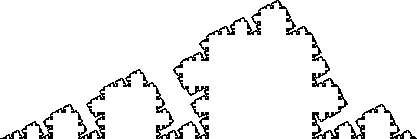
\includegraphics{fractal}
  \end{minipage}\par
  \begin{enumerate}
    \item Suppose you start with the straight line segment from $(0,0)$ to $(1,0)$. Draw the first two iterations of the fractal's construction.
    \item The dimension of the fractal is the unique solution $D$ to the equation
    \[\left(\frac 12\right)^D+\left(\frac 14\right)^D+\left(\frac 14\right)^D+\left(\frac 14\right)^D+\left(\frac 14\right)^D=1\]
    By observing that $\frac 14=\left(\frac 12\right)^2$, convert this to a quadratic equation in the variable $\alpha:=\left(\frac 12\right)^D$. Hence compute the dimension of the fractal.
       \item The dimension computed in part (b) is \emph{larger} than the dimension $\frac{\log 4}{\log 3}$ of the Koch curve. Explain what this means.
  \end{enumerate}


	\item Verify the details of Example \ref{ex:intervalcover}, including the computation of the limit.

	\item In Theorem \ref{thm:ifsdimension}, prove that $D$ exists and is unique.\\
	(\emph{Hint: You'll need the intermediate value theorem from calculus})
	
\end{enumerate}
\end{exercises}